 % !TeX spellcheck = it_IT
\documentclass[a4paper,12pt,titlepage]{report}
\pdfpagewidth
\paperwidth
\pdfpageheight
\paperheight
\usepackage[italian]{babel}
\usepackage{epsfig}
\usepackage{fancyhdr}
\usepackage{amsmath,amssymb}
\usepackage{amscd}
\usepackage{graphicx}
\usepackage[T1]{fontenc}
\usepackage[utf8]{inputenc}
\usepackage{version}
\usepackage[usenames,dvipsnames]{xcolor}
\usepackage{graphicx,color,listings}
\usepackage{hologo}
\frenchspacing
\usepackage{geometry}
\usepackage{rotating}
\usepackage{caption}
\captionsetup{labelformat=empty,textfont=sl}
\geometry{a4paper,tmargin=3cm,bmargin=3cm,lmargin=2.5cm,rmargin=2.5cm} \usepackage{multirow}
\usepackage{picture}
\textwidth16cm
\textheight24cm
\topmargin0mm
\headheight0mm
\oddsidemargin0mm
\evensidemargin0mm

\begin{document}
	\tableofcontents
\chapter{Introduction}
	Nowadays, many urban car manufactures are implementing the four-wheel steering system control on board. In this new vehicle generation, not only the front wheels are steerable but also the rear ones can be steered too. As a conseguence, the sistem will be characterized by a higher number of controlling inputs under equal number of states. This situation increases the maneuverability of the vehicle itself and provides the possibility of optimization or constraint satisfaction during the vehicle transfer between two definite boundaries.\\
	In this paper, we are going to present the kinetic and kinematic modeling of a four-wheel steering vehicle. Moreover, we will show our design procedure about the car optimal controller by means of the Linear Quadratic Regulator (LQR). The correctness of modeling and efficiency of the designed optimal controller is verified by the aid of a specific simulator we chose.\\
	The objective is to create a portable control that could be integrate in any vehicle and could work independently from the rest of the control systems of the vehicle, just getting as input the state of the vehicle and managing the steering angle of the rear wheels by itself.
\chapter{System Linearization}
	In this section we are going to describe the procedure we adopted in order to get the Linearized System. We will show our initial approximations and the main step we took, starting from the Non-Linear system equations up to the final equilibrium points. 
\section{Initial Approximations} \label{approx}	
	In order to modify the vehicle behaviour, we decided to act on the steering angles of the rear wheels. Thus, to elaborate that control system, we have considered a simplified vehicle model, characterized by the following approximations:
		\begin{itemize}
			\item[1.1] $ \gamma=\dot{\gamma}=0 $: flat plane condition leading to a null vertical acceleration;
			\item[1.2] $\vartheta = \phi = 0$ (Pitch and Roll angles, respectively): the vehicle is levelled with the North-West plane; 
			\item[1.3] No Wind and air drug contributions: the aerodynamic force components will be neglected;
		\end{itemize} 
\section{Non-Linear System}
	\subsection{1st Non-Linear Equation} 	
		Firstly, we obtained the $\chi$ and $\psi$ math definitions starting from the Vehicle Kinematics Equantions (both the Guidance and the Rotation ones) combined with the previous approximations. Than, through their geometrical relation, we got the following equation:
			\begin{equation}
				\beta_{u} = \chi - \psi
			\end{equation}
			Derivating the previous equation with respect to time we finally obtained the following statement:
			\begin{equation} \label{Betaudot}
				\dot{\beta}_{u} = \dot\chi - \dot\psi = 
				\begin{bmatrix}
				- \sin\beta_{u} & \cos\beta_{u}
				\end{bmatrix}
				\frac{1}{mV_{OB}}
				\begin{bmatrix}
				F_{wx}^{B} \\ F_{wy}^{B}
				\end{bmatrix}
				-\omega_{z}^{B}
			\end{equation}
	\subsection{2nd Non-Linear Equation}
		Starting from the Rotative Dynamic Equation and considering $\vartheta = \phi = 0$, we got the following relation:
			\begin{equation} \label{omegazdot}
				\dot{\omega}_{z}^{B} = \frac{1}{J_{z}} \tau_{z}^{B}
			\end{equation}
		The equations \ref{Betaudot} and \ref{omegazdot} represent, respectively, the 1st and the 2nd equations of the Non-Linear System.
\section{Linearization Parameters} 
	With the aim of achieve the proper linearized system for our model, we have analyzed the most critical variables affecting the vehicle itself. As a matter o facts, the overall system behaviour is influenced by many parameters, such as vehicle speed ($V_{OB}$), steering angle of both the front ($\delta_{wf}$) and rear ($\delta_{wr}$) wheels , the $\beta_{u}$ angle, and so on. \\
	In order to meet our final purpose, we fixed the following parameters as the reference ones for the linearization process:\\
		\begin{equation*}
			\tilde{x} =
			\begin{bmatrix}
			\beta_{u}^{B} \\\omega_{z}^{B}
			\end{bmatrix} = states \ variables
		\end{equation*}\quad
		\begin{equation*} 
			\tilde{u} =
			\begin{bmatrix}
			\delta_{wr}^{B} 
			\end{bmatrix} = control \ variables
		\end{equation*}\quad
		\begin{center}
			$ y = output \ variable $	
		\end{center}
			\begin{comment}
			\begin{equation*} 
				\tilde{d} =
				\begin{bmatrix}
				\delta_{wf}^{B} 
				\end{bmatrix} = disturbance \ variables
			\end{equation*}
			\end{comment}
\section{Linearization Point} 
	We chose to linearized our four-wheel steering control system around a straight trajectory of the vehicle. Doing so, we will accept even all those conditions which differ in a way from the previous one. In order to achieve this result, we fixed the following linearization point:
		\begin{equation*}
			\begin{cases}
				\beta_{u} = \omega_{z} = 0
			\end{cases}
		\end{equation*}
\section{Errors Definition}
	Computing the errors means evaluate the dynamic of parameters. To make sure we fully clarify what we are going to do, let's define the base values of each error equation (there follow the ones related to the \textit{states} variable):
		\begin{itemize}
			\item[$\bullet$] $x$ = current state vlue;
			\item[$\bullet$] $x_{0}$ = equilibrium point;
			\item[$\bullet$] $\tilde{x}$ = small variation of current state.
		\end{itemize}
	Once it has been figured out, there follow the error evaluation for all the considered variables.
		\begin{equation*}
			\begin{cases}
				x = x_{0} + \tilde{x} \\
				u = u_{0} + \tilde{u} \\
				%d = d_{0} + \tilde{d} \\
			\end{cases}
		\end{equation*}
	Than, if we simply compute the equivalent time-derivative of each statement, we get:
		\begin{equation*}
			\begin{cases}
				\dot{x} = \dot{x_{0}} + \dot{\tilde{x}} \\
				\dot{u} = \dot{u_{0}} + \dot{\tilde{u}} \\
				%\dot{d} = \dot{d_{0}} + \dot{\tilde{d}} \\
			\end{cases}
		\end{equation*}
	Let's compute the \textit{states} relation.\\
	Due to our linearization point, we can rightly say $x_{0} = 0 $, so its time derivative becomes zero as well.
		\begin{equation} \label{matrices structure}
			\begin{split}
				\dot{x}  = \dot{\tilde{x}} &= f(x_{0}+\tilde{x},u_{0}+\tilde{u})\approx \\
				&\approx f(x_{0}+u_{0}) + \frac{\partial f}{\partial x} |_{(x_{0},u_{0})} \tilde{x} + \frac{\partial f}{\partial u} |_{(x_{0},u_{0})} \tilde{u} = \\
				&= 0 + A \tilde{x} + B_{1} \tilde{u} 
			\end{split}
		\end{equation}
	Finally, from the equation \ref{matrices structure}, we obtained the origin of each matrix of our system. Inside the next paragraph we are going to elaborate all the partial derivatives within the equation \ref{matrices structure} in order to find each element for all the matrices.
\section{Linearized System} 
	Let's begin showing the final Linear Time-Invariant System we got:
		\begin{equation} \label{LTI}
			\begin{cases}
				\dot{\tilde{x}} = A \tilde{x} + B_{1}\tilde{u} \\
				y = C\tilde{x} 
			\end{cases}
		\end{equation}
	In the next steps, we are going to analyze each matrix appearing within the system \ref{LTI} and the processes we followed to achieve them.
	\subsection{Forces and Momentums}
		Aiming at describing the vehicle behaviour in a specific situation, we should take into account both the forces and momentums acting on it. \\ Regarding the overall \textit{Forces} typically applied to a generic vehicle, it is possible to split them into three main components: the \textit{gravity} force, the \textit{tire-wheels} forces and the \textit{aerodynamic} ones. In order to simplify our model, as previously said, we have considered some general approximations (see section \ref{approx}, page \pageref{approx}). We will report below the force-related ones:
		\begin{itemize}
			\item \textit{Aerodynamic} forces are negligible;
			\item Null vertical acceleration leads to zero \textit{gravity} force.
		\end{itemize}
		Given these assumptions, we have obtained a system characterized only by the \textit{tire-wheels} forces (from now on only "\textit{wheels} forces"). Moreover, since the vertical acceleration is negligible, we have considered only the x and y components of those forces. \\ Generally, the x-component (\textit{Longitudinal} member) is the sum of both rolling and friction resistances, while the y-one (\textit{Side} member) is only due to friction resistance. 
		Therefore, for each tire-wheel system of the vehicle, we have to eavluate both the components. \\
		There follow the \textit{wheels} forces acting, respectively, along the x and y-axis of the i-th tire-wheel system:
			\begin{equation} \label{split e roll}
				\begin{cases}
					F_{wx} = F_{Split} + F_{Rolling} = F_{wz} \mu_{L} + F_{wz} C_{R} \\
					F_{wy} = F_{Split} = F_{wz} \mu_{S}
				\end{cases}
			\end{equation}
		It is important to emphasise that the relation \ref{split e roll} is true for the i-th wheel. In order to achieve the whole \textit{wheels} force acting over the entire vehicle, we should consider it four times. \\ The \textit{Friction Coefficient}, $ \mu $, is defined as follow:
			\begin{equation}
				\mu = \mu(\lambda_{TOT})
			\end{equation}
		Moreover, we can specify the \textit{Friction Coefficients} related to both the Longitudinal and the Side slip directions as follow:
			\begin{equation}
				\begin{cases}
					\mu_{L} = \mu(\lambda_{TOT}) \frac{\lambda_{L}}{\lambda_{TOT}}\\
					\mu_{S} = \mu(\lambda_{TOT}) \frac{\lambda_{S}}{\lambda_{TOT}}
				\end{cases}
			\end{equation}
		The \textit{Slip} ratio, instead, is responsible to the friction resistance and it is defined by:
			\begin{equation}
			\lambda_{TOT} = \sqrt{\lambda_{L}^{2} + \lambda_{S}^{2}} \leq 1
			\end{equation}
		Finally, merging all those concepts together, we arrived to the following notation:	
			\begin{equation} \label{Force 1st part}
				\begin{bmatrix}
					F_{wx} \\
					F_{wy}
				\end{bmatrix}^{W} = 
				F_{wz}^{W}
				\begin{bmatrix}
					\mu_{L} \\
					\mu_{S}
				\end{bmatrix} = 
				F_{wz}^{W}
				\begin{bmatrix}
					\frac{\lambda_{L}}{\lambda_{TOT}} \\
					\frac{\lambda_{S}}{\lambda_{TOT}}
				\end{bmatrix}
				\mu(\lambda_{TOT})	
			\end{equation}
		From the geometric point of view, in terms of reference frames, we can define the \textit{wheels} forces with the following notation:
			\begin{equation} \label{Force 2nd part}
				\begin{bmatrix}
					F_{wx} \\
					F_{wy}
				\end{bmatrix}^{B} =	
				R_{BW}
				\begin{bmatrix}
					F_{wx} \\
					F_{wy}
				\end{bmatrix}^{W} =
				\begin{bmatrix}
					\cos\delta_{w} & -\sin\delta_{w} \\
					\sin\delta_{w} & \cos\delta_{w}
				\end{bmatrix}
				\begin{bmatrix}
					F_{wx} \\
					F_{wy}
				\end{bmatrix}^{W}
			\end{equation}
		Combining together the equations \ref{Force 1st part} and \ref{Force 2nd part}, we obtain the final expression for the \textit{wheels} forces we employed:
			\begin{equation} \label{Forces}
				\begin{bmatrix}
					F_{wx} \\
					F_{wy}
				\end{bmatrix}^{B} =	
				\begin{bmatrix}
					\cos\delta_{w} & -\sin\delta_{w} \\
					\sin\delta_{w} & \cos\delta_{w}
				\end{bmatrix}
				\frac{F_{wz}^{W} \mu(\lambda_{TOT})}{\lambda_{TOT}}
				\begin{bmatrix}
					\lambda_{L} \\
					\lambda_{S}
				\end{bmatrix}
			\end{equation}
		By processing the above equation \ref{Forces}, we got the two following relations:
			\begin{equation} \label{F_{wy}}
			\begin{split}
				F_{wy}^{B} = 2 [F_{wz}^{W} \mu_{S}\sin\delta_{wr} + (F_{wz}^{W} \mu_{L} + F_{wz}^{W} C_{R}) \cos\delta_{wr}] + \\ + 2 [F_{wz}^{W} \mu_{S}\sin\delta_{wf} + (F_{wz}^{W} \mu_{L} + F_{wz}^{W} C_{R})\cos\delta_{wf}] 
			\end{split}
			\end{equation}
			\begin{equation} \label{F_{wx}}
			\begin{split}
				F_{wx}^{B} = 2 [(F_{wz}^{W} \mu_{L} + F_{wz}^{W} C_{R})\cos\delta_{wr} - F_{wz}^{W} \mu_{S}\sin\delta_{wr}] + \\ + 2 [(F_{wz}^{W} \mu_{L} + F_{wz}^{W} C_{R})\cos\delta_{wf} - F_{wz}^{W} \mu_{S}\sin\delta_{wf}] 
			\end{split}
			\end{equation}
		Regarding the overall \textit{Momentums} affecting the vehcile behaviour, we simply considered the ones coming from the forces we took into account. By multiplying them by their own arms we obtained the following general statement:
			\begin{equation}
				\sum \tau^{B} = \sum r^{B} \sum F_{tire-wheels}^{B}
			\end{equation}
		The evolution of the previous equation, considering only our paramenters of interest, is the following one:  
			\begin{equation}
				\begin{split}
					\tau^{B} &= -\omega_{z}\sum_{i=1}^{4} F_{wz_{i}}^{w} \frac{\mu(\lambda_{TOT_{i}})}{\lambda_{TOT_{i}} V_{max}} (r_{x_{i}}^{2} + r_{y_{i}}^{2})- \\ &- V_{OB}\sum_{i=1}^{4} F_{wz_{i}}^{w} \frac{\mu(\lambda_{TOT_{i}})}{\lambda_{TOT_{i}} V_{max}} (- r_{y_{i}} \cos \beta_{u} + r_{x_{i}} \sin\beta_{u})+ \\ &+ ... 
				\end{split}	
			\end{equation}
		where "$ ... $" means all those components which do not depend neither on $\beta_{u}$ nor $\omega_{z}$.
	\subsection{Matrix A}
		Before showing aech element of matrix A, we  need to remind that we started from the two non-linear equations previoulsy described: \ref{Betaudot} and \ref{omegazdot}, respectively. Moreover, since we started with two \textit{state} variables, we have obtained a matrix A $\in M_{2X2}$.\\ There follow the four elements of matrix A:
			\begin{equation} \label{a11}
				\begin{split}
					a_{11} &= \frac{\partial\dot{\beta}_{u}^{B}}{\partial\beta_{u}} = \\ 
					&= \frac{1}{mV_{OB}}
					\begin{bmatrix}
					- \cos\beta_{u} & -\sin\beta_{u}
					\end{bmatrix}
					\begin{bmatrix}
					F_{wx}^{B} \\ F_{wy}^{B}
					\end{bmatrix}
					+ \frac{1}{mV_{OB}} 
					\begin{bmatrix}
					- \sin\beta_{u} & \cos\beta_{u}
					\end{bmatrix}
					\begin{bmatrix}
					\frac{\partial F_{wx}}{\partial\beta_{u}}^{B} \\ \frac{\partial F_{wy}}{\partial\beta_{u}}^{B}
					\end{bmatrix}
				\end{split}
			\end{equation} 
			\begin{equation} \label{a12}
				a_{12} = \frac{\partial\dot{\beta}_{u}^{B}}{\partial\omega_{z}} = -1
			\end{equation} 
			\begin{equation} \label{a21}
				a_{21} = \frac{\partial\dot{\omega}_{z}^{B}}{\partial\beta_{u}} = \frac{1}{J_{z}} \frac{\partial\tau_{z}^{B}}{\partial\beta_{u}} \vert_{\beta_{u}=0} = -\frac{1}{J_{z}} V_{0B} \sum\limits_{i=1}^4 F_{wz_{i}}^{w} \mu(\lambda_{0}) \frac{1}{v_{max}}r_{x_{i}}
			\end{equation}
			\begin{equation} \label{a22}
				a_{22} = \frac{\partial\dot{\omega}_{z}^{B}}{\partial\omega_{z}} = \frac{1}{J_{z}} \frac{\partial\tau_{z}^{B}}{\partial\omega_{z}} = -\frac{1}{J_{z}}\sum\limits_{i=1}^4 F_{wz_{i}}^{w} \mu(\lambda_{0}) \frac{1}{v_{max}} (r_{x_{i}}^{2} + r_{y_{i}}^{2}) 
			\end{equation}
	Finally, joining together all the previous components, we got the following matrix A form:
		\begin{equation}
			A=
			\begin{bmatrix}
				\frac{\partial\dot{\beta}_{u}^{B}}{\partial\beta_{u}^{B}} & \frac{\partial\dot{\beta}_{u}^{B}}{\partial\omega_{z}^{B}} \\
				\frac{\partial\dot{\omega}_{z}^{B}}{\partial\beta_{u}^{B}} & \frac{\partial\dot{\omega}_{z}^{B}}{\partial\omega_{z}^{B}}
			\end{bmatrix} = 
			\begin{bmatrix}
				 -\frac{1}{mV_{0B}}\{F_{wx}^{B}\}  & -1  \\
				  -\frac{1}{J_{z}} V_{0B} \sum\limits_{i=1}^4 F_{wz_{i}}^{w} \mu(\lambda_{0}) \frac{1}{v_{max}}r_{x_{i}} &  -\frac{1}{J_{z}}\sum\limits_{i=1}^4 F_{wz_{i}}^{w} \mu(\lambda_{0}) \frac{1}{v_{max}} (r_{x_{i}}^{2} + r_{y_{i}}^{2}) 
			\end{bmatrix}
		\end{equation}
	\subsection{Matrix $B_{1}$} \label{B1}
		\begin{equation}
			B_{1}=
			\begin{bmatrix} 
				\frac{\partial\dot{\beta}_{u}^{B}}{\partial\delta_{r}^{B}} \\
				\frac{\partial\dot{\omega}_{z}^{B}}{\partial\delta_{r}^{B}}
			\end{bmatrix} = 
			\begin{bmatrix}
				-\frac{1}{mV_{0B}}\{-\sin\beta_{u}\frac{\partial F_{wx}^{B}}{\partial \delta_{wr}} + \cos\beta_{u}\frac{\partial F_{wy}^{B}}{\partial \delta_{wr}}\}  \\
				\frac{1}{J_{z}} \frac{\partial \tau_{z}^{B}}{\partial\delta_{wr}} = \frac{1}{J_{z}} \{ \sum\limits_{i=1}^4 C_{R}F_{wz_{i}}^{w} r_{x_{i}} + \sum\limits_{i=1}^4 F_{wz_{i}}^{w} \mu(\lambda_{0}) \frac{\omega_{i} r}{v_{max}}r_{x_{i}} \}
			\end{bmatrix}
		\end{equation} 
	In order to better clarify the equation \ref{B1}, there will follow the forces s partial derivatives components computed without imposing the initial conditions. By doing so, we kept all the parameters of interest inside these equations. In this way, we were able to study the vehicle behaviour simply by changing these parameters inside the model MATLAB code and analyzing the correspondent conseguences. \\ There will follow the x-relative partial derivatives formulas: 
		\begin{equation} \label{Fwx su deltaR }
			\begin{split}
				\frac{\partial F_{wx}^{B}}{\partial \delta_{wr}} &= 2 [\frac{\partial F_{wz}^{W}}{\partial \delta_{wr}} (\mu_{L}+C_{R}) \cos\delta_{wr} - F_{wz}^{W} (\mu_{L}+C_{R})\sin\delta_{wr} - \\
				&- \frac{\partial F_{wz}^{W}}{\partial \delta_{wr}} \mu_{S} \sin \delta_{wr} - F_{wz}^{W} \mu_{S}\cos\delta_{wr} - \frac{\partial F_{wz}^{W}}{\partial \delta_{wr}} \mu_{S} \sin \delta_{wf} + \frac{\partial F_{wz}^{W}}{\partial \delta_{wr}} (\mu_{L}+C_{R}) \cos\delta_{wf}]
			\end{split}
		\end{equation}
		\begin{equation} \label{Fwx su deltaF}
			\begin{split}
				\frac{\partial F_{wx}^{B}}{\partial \delta_{wf}} &= 2 [\frac{\partial F_{wz}^{W}}{\partial \delta_{wf}} (\mu_{L}+C_{R}) \cos\delta_{wr} - \frac{\partial F_{wz}^{W}}{\partial \delta_{wf}} \mu_{S} \sin \delta_{wr} + \frac{\partial F_{wz}^{W}}{\partial \delta_{wf}} - (\mu_{L}+C_{R}) \cos\delta_{wf} - \\
				&- F_{wz}^{W} (\mu_{L}+C_{R})\sin\delta_{wf}
				- \frac{\partial F_{wz}^{W}}{\partial \delta_{wf}} \mu_{S} \sin \delta_{wf} - F_{wz}^{W} \mu_{S}\cos\delta_{wf}]
			\end{split}
		\end{equation}
	The next two equations will be the y-relative ones:
		\begin{equation} \label{Fwy su deltaR}
			\begin{split}
				\frac{\partial F_{wy}^{B}}{\partial \delta_{wr}} &= 2 [\frac{\partial F_{wz}^{W}}{\partial \delta_{wr}} \mu_{S} \sin \delta_{wr} + F_{wz}^{W} \mu_{S}\cos\delta_{wf} + \frac{\partial F_{wz}^{W}}{\partial \delta_{wr}} (\mu_{L}+C_{R}) \cos\delta_{wr} + F_{wz}^{W}(\mu_{L}+C_{R}) \sin\delta_{wr}+ \\ &+ \frac{\partial F_{wz}^{W}}{\partial \delta_{wr}} \mu_{S} \sin \delta_{wf} + \frac{\partial F_{wz}^{W}}{\partial \delta_{wr}} (\mu_{L}+C_{R})\cos\delta_{wf}]
			\end{split}
		\end{equation}
		\begin{equation} \label{Fwy su deltaF}
			\begin{split}
				\frac{\partial F_{wy}^{B}}{\partial \delta_{wf}} &= 2 [\frac{\partial F_{wz}^{W}}{\partial \delta_{wf}} \mu_{S} \sin \delta_{wr} + \frac{\partial F_{wz}^{W}}{\partial \delta_{wf}} (\mu_{L}+C_{R}) \cos\delta_{wr} + \frac{\partial F_{wz}^{W}}{\partial \delta_{wf}} \mu_{S} \sin \delta_{wf}+ \\ &+ \frac{\partial F_{wz}^{W}}{\partial \delta_{wf}} (\mu_{L}+C_{R})\cos\delta_{wf} - F_{wz}^{W} (\mu_{L}+C_{R}) \sin\delta_{wf}]
			\end{split}
		\end{equation}
	\begin{comment}
	\subsection{Matrix $B_{2}$}
	Considering that our \textit{disturbance} variable ($\delta_{wf}$) is always a steering angle as the \textit{control} one ($\delta_{wr}$), the processing phase of Matrix $B_{2}$ was exactly the same as the Matrix $B_{1}$ one. \\ The final result is reported down here:
		\begin{equation}
			B_{2}=
			\begin{bmatrix}
			\frac{\partial\dot{\beta}_{u}^{B}}{\partial\delta_{f}^{B}} \\
			\frac{\partial\dot{\omega}_{z}^{B}}{\partial\delta_{f}^{B}} 
			\end{bmatrix} =
			\begin{bmatrix}
			 -\frac{1}{mV_{0B}}\{-\sin\beta_{u}\frac{\partial F_{wx}^{B}}{\partial \delta_{wf}} + \cos\beta_{u}\frac{\partial F_{wy}^{B}}{\partial \delta_{wf}}\} \\
		\frac{1}{J_{z}} \frac{\partial \tau_{z}^{B}}{\partial\delta_{wf}} = \frac{1}{J_{z}} \{ \sum\limits_{i=1}^4 C_{R}F_{wz_{i}}^{w} r_{x_{i}} + \sum\limits_{i=1}^4 F_{wz_{i}}^{w} \mu(\lambda_{0}) \frac{\omega_{i} r}{v_{max}}r_{x_{i}} \}
			\end{bmatrix}
		\end{equation}
	For the elaboration of all the partial derivatives above, refer to subsection \ref{B1}.
	\end{comment}
	\subsection{Matrix C}
	The choice of matrix C was dictated by the math relationship among the x-variable (\textit{states}) and the y-one (\textit{output}) of the system \ref{LTI}, pag. \pageref{LTI}. With the aim of simplifying our system model, we chose the \textit{Identity} matrix to connect these system variables together. \\ In our case, according to both x and y-matrix sizes, we have obtained a matrix C $\in M_{2X2}$.
		\begin{equation}
		C = 
		\begin{bmatrix}
			1 & 0 \\
			0 & 1
		\end{bmatrix}
		\end{equation}
\chapter{System Analysis: Stability, Observability and Reachability}
	Within the current chapter, we are going to describe how we analyzed our system in terms of both observability and reachability. In particular, we will firstly show how we proved the system stability and, finally, we will exhibit the equilibium points we got.
\section{System Stability} 
	From the theory, it is possible to define "stable" a Linear Time Invariant (LTI) system IF ONLY the eigenvalues of matrix A are strictly negative.
\section{System Reachability}
\section{Equilibrium Points}
	With the purpose of getting the equilibrium points of both $\beta_{u}$ and $\omega_{z}$, we have imposed the following condition to our LTI system:
		\begin{equation} \label{Equilibrium condition}
			\begin{bmatrix}
				\dot{\tilde{\beta_{u}}} \\
				\dot{\tilde{\omega_{z}}}
			\end{bmatrix} =
			\begin{bmatrix}
				0 \\
				0
			\end{bmatrix} = A
			\begin{bmatrix}
				\tilde{\beta_{u}} \\
				\tilde{\omega_{z}}
			\end{bmatrix} 
			B_{1}[\tilde{\delta_{wr}}] B_{2}[\tilde{\delta_{wf}}]
		\end{equation}
	The equation \ref{Equilibrium condition} is directly given by the "equilibrium point" definition: \textit{to be considered an equilibrium poit, the current parameter must have a zero time derivative}. If the matrix A is invertible, we can write the following statement:
		\begin{equation} \label{eq points}
			\begin{bmatrix}
				\tilde{\beta_{uEQ}} \\
				\tilde{\omega_{zEQ}}
			\end{bmatrix} = 
			A^{-1}[-B_{1} \tilde\delta_{wr} - B_{2} \tilde\delta_{wf}]
		\end{equation}
	From the equation \ref{eq points} we got our equilibrium points, $\beta_{uEQ}$ and $\omega_{zEQ}$.
\chapter{Optimal Control Design}
	Inside this chapter, we are going to show the control system we designed for our application. This phase has been the most complex one for different reasons. Generally speaking, the design of a specific control law for each physical system depends by many factors, having different levels of influence. For this reason, we tried to design the best possible control law by considering more the most important elements and neglecting and/or minimizing the ones with a low impact. As a conseguence, this step required us lots of time to be fully accomplished.\\
	First of all, we described our vehicle model through the Matlab Software. We have both provided its physical description and initialized all those variables able to influence its behcaviour. Than we thought about the model simulator in order to have the simulation environment inside with test our changes. Moreover, with the aim of controlling the steering angle of the rear wheels, we dsigned the optimal control law for our system. Finally, we merged the simulator and the control low together in Simulink. \\
	The next sections will contain a more accurated description of those step we just introduced.
\section{Vehicle Model design}
	It was the first step of the entire procedure we realized. The current section was purely related to achieve a real vehicle model, characterized by all the  parameters needed to simulate and analyze the car behaviour. As a matter of facts, we have to remember that our goal was to control the vehicle working conditions by means of the rear steering angle actuation. We could reach the previous purpose only with a real representation of the vehicle itself, made up of its main technical and physical parameters.\\
	We have implemented such a model on Matlab, describing the automobile features inside a live script. Firstly, we have initialized all the control variables needed for the following computations. Than, we fixed some vehicle's physical parameters, such as mass, wheels position with respect to centre of gravity of the car, and so on. At the end of current section, there will be an extract from our Matlab model.
		\begin{figure} %\label{key}
			\centering
	%		\includegraphics[scale=0.5,width=0.25\textheight]{NOME}
	%		\caption{text}
		\end{figure}
\section{Control Law design}
	This step was the most critical one because of its close correlation with the project purpose itself. Our starting object was to develop a control law ables to act over the steering angle of the rear wheels, $\delta_{wr}$. There will follow a step-by-step description of our procedure.
	\subsection{Cost Function $J$ Analysis}
		Starting from the theory, we studied the real meaning of "Cost Function" and its elements. The function's goal is to design a control system, $u$, ables to minimize the function $J$ itself. In a nutshell, if a certain condition is strongly desired, we have to associate to it a low cost, and viceversa. \\
		There follow the linear quadratic form of the cost function $J$ for a general LTI system:
			\begin{equation}
				J = x^{T}(t_{f}) S_{f} x(t_{f})\int_{t_{0}}^{t_{f}} e^{T} Q e + u^{T} R u \ dt
			\end{equation}
		where:
			\begin{itemize}
				\item $e$ represents a linear combination of \textit{states} x;
				\item $u$ represents the control law;
				\item $ [t_{0},t_{f}] $ represents the time spain in which we evaluated our cost function J;
				\item $ S_{f} = S_{f}^{T} \geq0 $ represents the cost associated to the state once it is evaluated in $t=t_{f}$, so "how much far i am from the origin";
				\item $ Q=Q^{T}\geq 0 $ and $ R=R^{T}\geq 0 $ represent, respectively, the costs for having $e\neq0$ and $u\neq0$, during the time span.
			\end{itemize}
	\subsection{Q and R Matrices}
		We could reach our final goal, in terms of meaningful imposed rear steering angle, through the "tuning" process of matrices $Q$ and $R$. For what concern the matrix $S$, we set it equal to zero ..?..	
	\subsection{K multiplier}
		Following the theory of optimal control we should extract one single K matrix around the linearization point. This made our working condition very limited, because in choosing a linearization point we would have to choose one single steering angle and angular velocity, thus restricting the range of validity of our system around a certain kind of curve, that initially was as specific as a straight trajectory ($\omega_{z}=0$).
		This reason lead us towards the consideration of extracting not one matrix for K, but a whole range of values, based on two inputs from the driver:
\begin{itemize}
	\item front steering angle $\delta_{wf}$
	\item speed $V_0$
\end{itemize}	
		This extraction is not done in real time, due to the relatively high computational load of performing an LQR algorithm, it is instead done only once at the startup of the system (now that we are in prototypation phase, later on it will only be performed once and for all). After this initial computations made at some discrete linearization points, the results will be stored in lookup tables, at runtime the only workload for the microcontroller will be to take as input the actual state of the machine, specifically the two input parameters written in the bullet list here above and perform matrix multiplcation as usual.//
		Obviously, given the discrete nature of the lookup table, it will not be possible to have a perfect match for the actual disturbances of the vehicle that span across a continuous space, so we will have to approximate to the nearest point of linearization. It will be anyway a better approximated solution with respect to a system with a single linearization point and a single K.//
		Another reason why we have devoted one script for the extraction of K matrices and another one for the computation of realtime control is that you can't generate C code using matlab coder or even a simulink block with Matlab code containing the lqr algorhytm present in the control system toolbox. We needed to keep it separate.
\chapter{Vehicle Simulator}
	In order to have the most realistic simulation possible, we decided not to design our own discrete time non -linear simulator, instead we utilize a Matlab toolbox called "vehicle dynamics" and integrate it into our project. It is a Simulink based toolbox that has some useful blocks for every vehicle control system (like ESP and cruise control) and for simulations of parts of the vehicle (like engine, suspensions and transmission). 
	It has been particularly useful also because it offered already pre-built reference applications, for constant radius steering, double lane change and similar situations, coupled with a system of scopes that allowed us to visualize the data that we needed. We built our application starting from the constant radius steering, adding our control system for the rear wheels together with the other controls.
	\paragraph{Driver inputs simulation}
	The Vehicle Dynamics blockset also offers a block called "predictive driver" that, given a reference trajectory, tries to maintain it acting on the accelerator pedal or on the steering wheel. After some trials we verified that it was not designed with the knowledge of steerable rear wheels, thus leading to instability of its prediction system, we had to disable it and bypass it, giving directly a fixed front steer angle $\delta_{wf}$ and speed.
	\paragraph{Graphic engine}
	This blockset also includes a graphic tool, in order to view in a 3D environment the movements of the vehicle, it can be enabled or disabled based on the graphics capabilities of the system on which the software is working on. This tool is based upon Unreal Engine.
\chapter{Final Results}
Per ora solamente mandala:\\
\begin{figure}[!h]
\centering
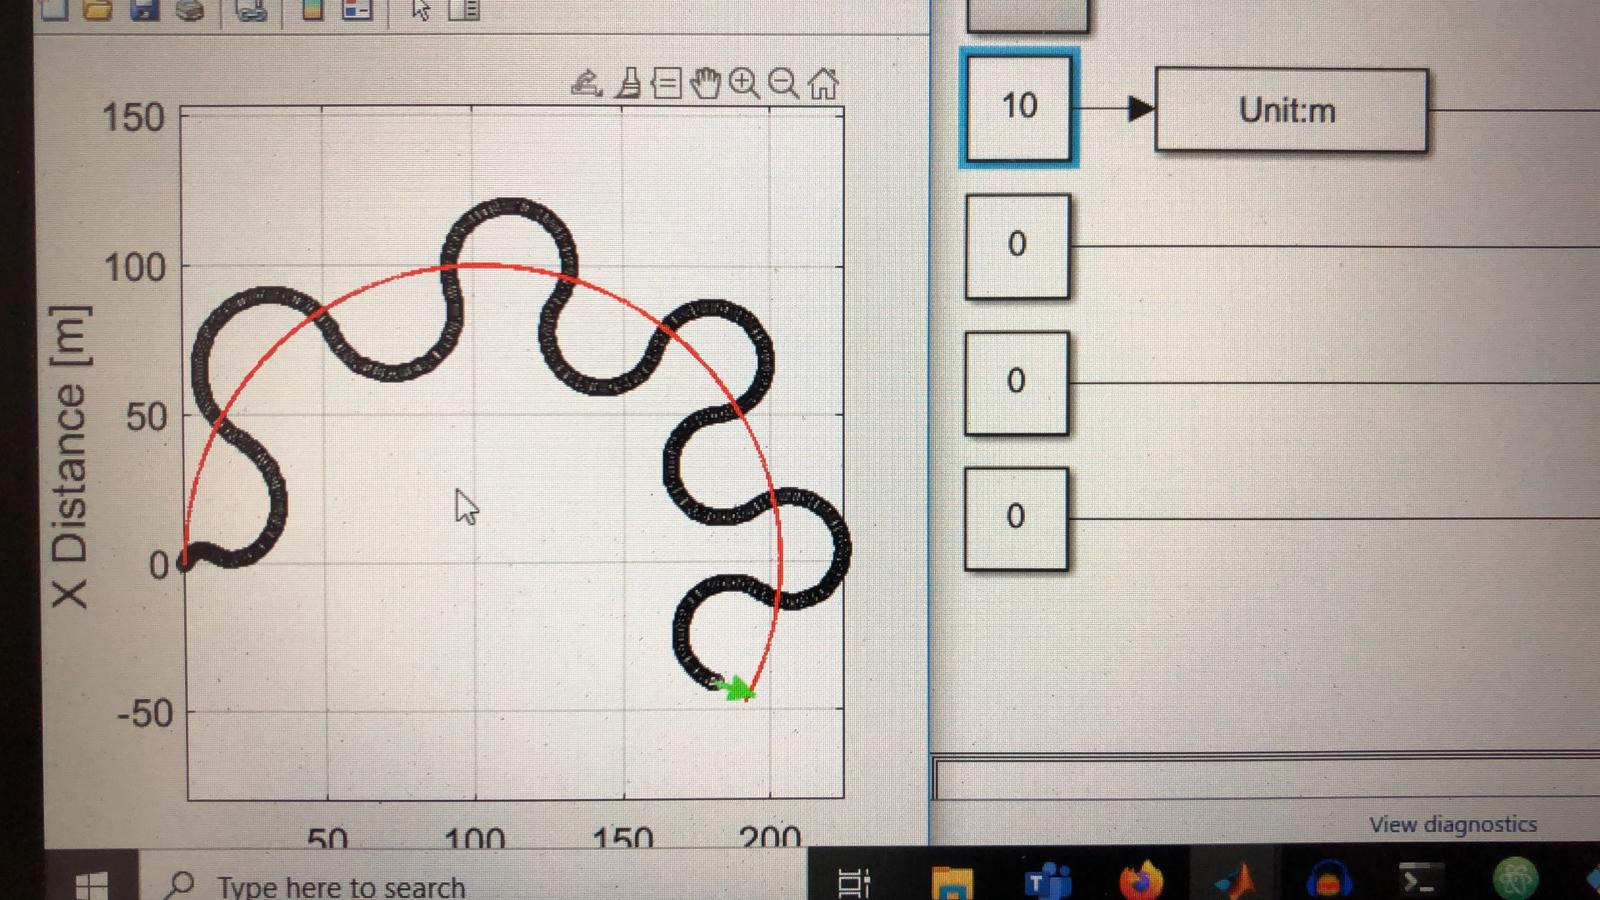
\includegraphics[scale=0.2]{mandala1}
\caption{Tipica traiettoria a mandala dovuta al predictive driver ignaro di tutto}
\end{figure}
\end{document}